%%%%%%%%%%%%%%%%%%%%%%%%%%%%%%%%%%%%%%%%%%%%%%%%%%%%%%%%%%%%%%%%%
% MUW Presentation
% LaTeX Template
% Version 1.0 (27/12/2016)
%
% License:
% CC BY-NC-SA 4.0 (http://creativecommons.org/licenses/by-nc-sa/3.0/)
%
% Created by:
% Nicolas Ballarini, CeMSIIS, Medical University of Vienna
% nicoballarini@gmail.com
% http://statistics.msi.meduniwien.ac.at/
%
% Customized for UAH by:
% David F. Barrero, Departamento de Automática, UAH
%%%%%%%%%%%%%%%%%%%%%%%%%%%%%%%%%%%%%%%%%%%%%%%%%%%%%%%%%%%%%%%%%

\documentclass[10pt,compress,xcolor=table]{beamer} % Change 10pt to make fonts of a different size
\mode<presentation>
\usepackage{ragged2e}
\usepackage[spanish]{babel}
\usepackage{fontspec}
\usepackage{tikz}
\usepackage{etoolbox}
\usepackage{listings}
% Para las checkmarks and crossmarks in latex
\usepackage{amssymb}% http://ctan.org/pkg/amssymb
\usepackage{pifont}% http://ctan.org/pkg/pifont
\newcommand{\cmark}{\ding{51}}%
\newcommand{\xmark}{\ding{55}}%
\usepackage{color}
%\usepackage[table,xcdraw]{xcolor}
\usepackage{wasysym}
\usepackage{graphicx}
\tikzstyle{Caja1} = [green,very thick,rounded corners,fill=white, fill opacity=0.5]
\tikzstyle{Texto1} = [fill=white,thick,shape=circle,draw=black,inner sep=2pt,font=\sffamily,text=black]
\tikzstyle{Texto2} = [fill=white,thick,shape=rectangle,draw=black,inner sep=2pt,font=\sffamily,text=black]
\tikzstyle{Texto3} = [fill=white,thick,shape=circle,draw=black,inner sep=2pt,font=\sffamily,text=black]
% Cuadros de diagrama
\tikzstyle{rectvioleta} = [rectangle, rounded corners, text centered, draw=black, fill=blue!10]
\tikzstyle{rectnaranja} = [rectangle, rounded corners, minimum width=2cm, minimum height=1cm, text centered, draw=black, fill=orange!10]
\tikzstyle{romborosa} = [diamond, aspect=3, minimum width=3cm, minimum height=1cm, text centered, draw=black, fill=red!10]
\tikzstyle{rectverde} = [rectangle, rounded corners, minimum width=2cm, minimum height=1cm, text centered, draw=black, fill=green!10]
\tikzstyle{rectamarillo} = [rectangle, rounded corners, minimum width=2cm, minimum height=1cm, text centered, draw=black, fill=yellow!10]
% Flechas
\tikzstyle{arrow} = [thick,->,>=stealth]
\lstdefinestyle{P4-color}
	{
  	breaklines=true,
  	language=C,
  	keywordstyle=\bfseries\color{green!40!black},
  	commentstyle=\itshape\color{purple!40!black},
  	identifierstyle=\color{blue},
  	stringstyle=\color{orange},
  	morekeywords={%
      action, algorithm, apply, attributes, bytes,
      calculated_field, control, counter, current, default, direct,
      drop, else, false, field_list, field_list_calculation, fields,
      header, header_type, hit, if, input, instance_count, last, latest,
      layout, length, mask, max_length, metadata, meter, min_width, miss
      output_width, packets, parse_error, parser, parser_exception, payload,
      primitive_action, register, result, return, saturating, select,
      signed, static, switch, true, type, update, valid, verify, width, macAddr_t, egressSpec_t}
    }


\usetheme{UAH}
\usecolortheme{UAH}
\setbeamertemplate{navigation symbols}{} 
\setbeamertemplate{caption}[numbered]

%%%%%%%%%%%%%%%%%%%%%%%%%%%%%%%%%%%%%%%%%%%%%%%%%%%%%%%%%%%%%%%%%
%% Presentation Info
\title[Trabajo Fin de Grado]{Diseño y estudio de dispositivos IoT integrados en entornos SDN}
\author{David Carrascal Acebrón}
\institute{Departamento de Automática}
\date{16 de Julio del 2020}
%%%%%%%%%%%%%%%%%%%%%%%%%%%%%%%%%%%%%%%%%%%%%%%%%%%%%%%%%%%%%%%%%


%%%%%%%%%%%%%%%%%%%%%%%%%%%%%%%%%%%%%%%%%%%%%%%%%%%%%%%%%%%%%%%%%
%% Descomentar para habilitar barra de navegación superior
\setNavigation
%%%%%%%%%%%%%%%%%%%%%%%%%%%%%%%%%%%%%%%%%%%%%%%%%%%%%%%%%%%%%%%%%

%%%%%%%%%%%%%%%%%%%%%%%%%%%%%%%%%%%%%%%%%%%%%%%%%%%%%%%%%%%%%%%%%
%% Configuración de logotipos en portada
%% Opacidad de los logotipos
\newcommand{\opacidad}{1}
%% Descomentar para habilitar logotipo en pié de página de portada
%\renewcommand{\logoUno}{img/isg.png}
%% Descomentar para habilitar logotipo en pié de página de portada
%\renewcommand{\logoDos}{img/CCLogo.png}
%% Descomentar para habilitar logotipo en pié de página de portada
%\renewcommand{\logoTres}{img/ALogo.png}
%% Descomentar para habilitar logotipo en pié de página de portada
%\renewcommand{\logoCuatro}{img/ELogo.png}
%%%%%%%%%%%%%%%%%%%%%%%%%%%%%%%%%%%%%%%%%%%%%%%%%%%%%%%%%%%%%%%%%


\footlineA

%%%%%%%%%%%%%%%%%%%%%%%%%%%%%%%%%%%%%%%%%%%%%%%%%%%%%%%%%%%%%%%%%

\begin{document}

%%%%%%%%%%%%%%%%%%%%%%%%%%%%%%%%%%%%%%%%%%%%%%%%%%%%%%%%%%%%%%%%%
% Use this block for a blue title slide with modified footline
{\titlepageBlue
	% Content
    \begin{frame}
        \titlepage
    \end{frame}
}

%%%%%%%%%%%%%%%%%%%%%%%%%%%%%%%%%%%%%%%%%%%%%%%%%%%%%%%%%%%%%%%%%
% Comment/Uncomment these lines for an automatically generated outline.
{\disableNavigation{white}
    \begin{frame}{Índice}
        \tableofcontents
    \end{frame}
}



\addtocounter{framenumber}{-1} %To control the number in which numbering begins

%%%%%%%%%%%%%%%%%%%%%%%%%%%%%%%%%%%%%%%%%%%%%%%%%%%%%%%%%%%%%%%%%
\section{Introducción}
\begin{frame}{Introducción}
\begin{block}{Dos tecnologías...}
El Internet de las Cosas y las Redes Definidas por Software, son tecnologías emergentes que
desde hace unos años están revolucionando los paradigmas sobre los modelos de redes comunicaciones establecidos en el pasado.\vspace{0.2cm}
\end{block}
\vspace{0.2cm}
Las redes SDN $ \Rightarrow $ extraer el plano de control de los dispositivos intermedios de procesamiento de la red, unificándolo en \textbf{controladores}.\vspace{0.2cm} 
\begin{itemize}
    \item La administración de red una tarea más \textbf{centralizada} y \textbf{flexible}.
\end{itemize} \vspace{0.2cm}

El IoT  $ \Rightarrow $ interconectar billones de objetos entre sí a través de Internet. 
\end{frame}



%%%%%%%%%%%%%%%%%%%%%%%%%%%%%%%%%%%%%%%%%%%%%%%%%%%%%%%%%%%%%%%%%
\subsection{Tipos de integración}
\begin{frame}{Introducción}{Tipos de integración}

\begin{columns}

  \begin{column}{0.5\textwidth}
    \begin{figure}
      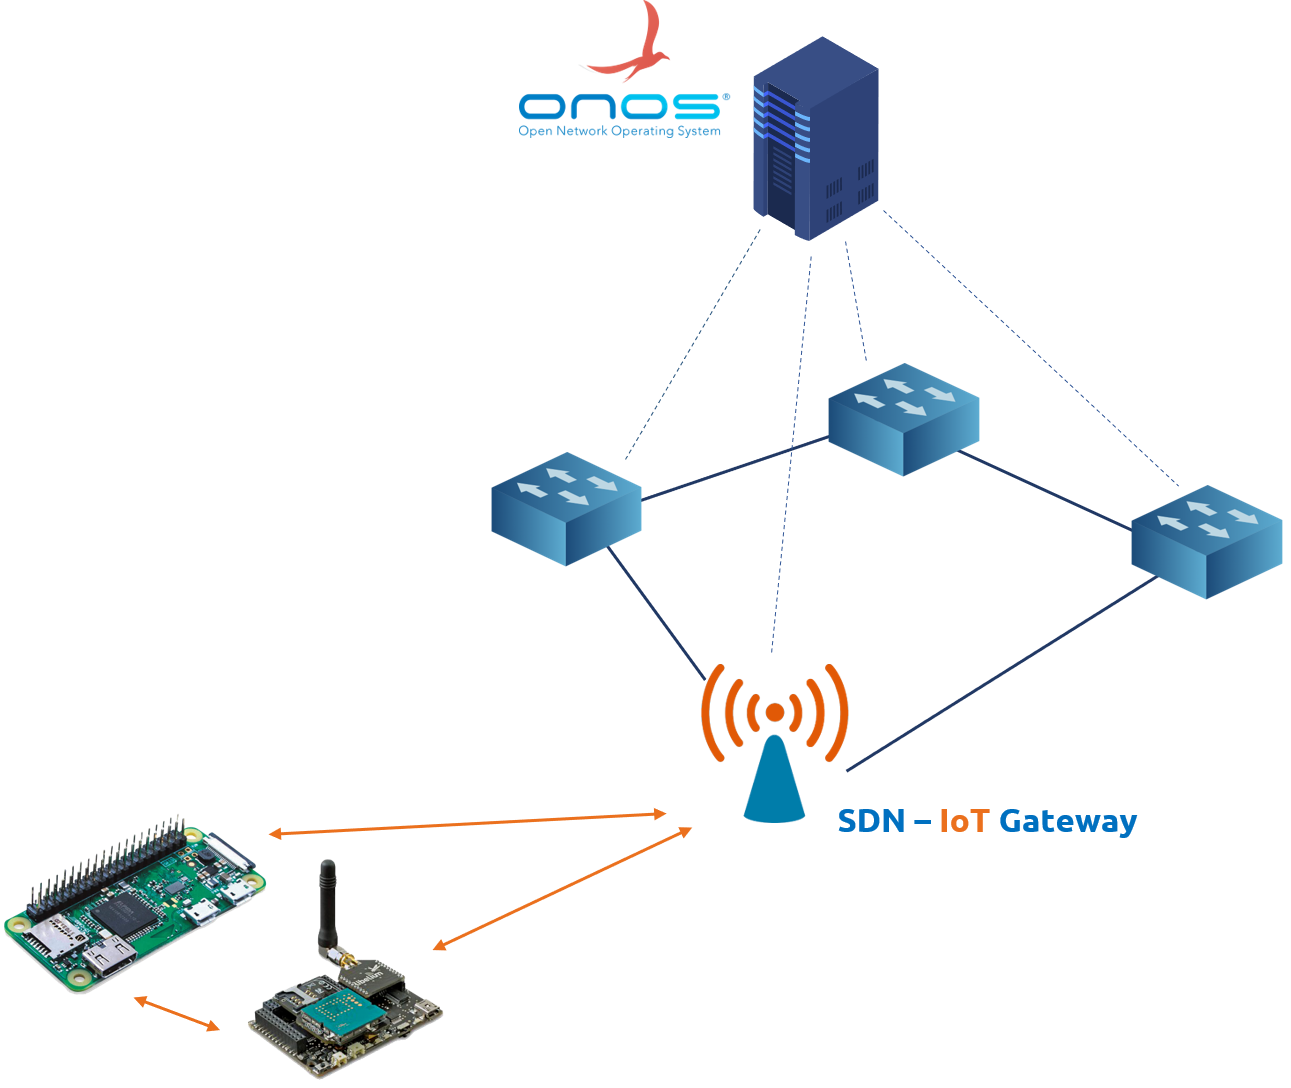
\includegraphics[width=0.8\textwidth]{img/sdn_iot.png}
      \caption{ Integración parcial de dispositivos IoT en el core SDN}
      \label{fig:sdn_iot}
    \end{figure}
        
  \end{column}
  \vrule\hspace{0.4cm}
  \begin{column}{0.5\textwidth}  %%<--- here
     \begin{figure}
      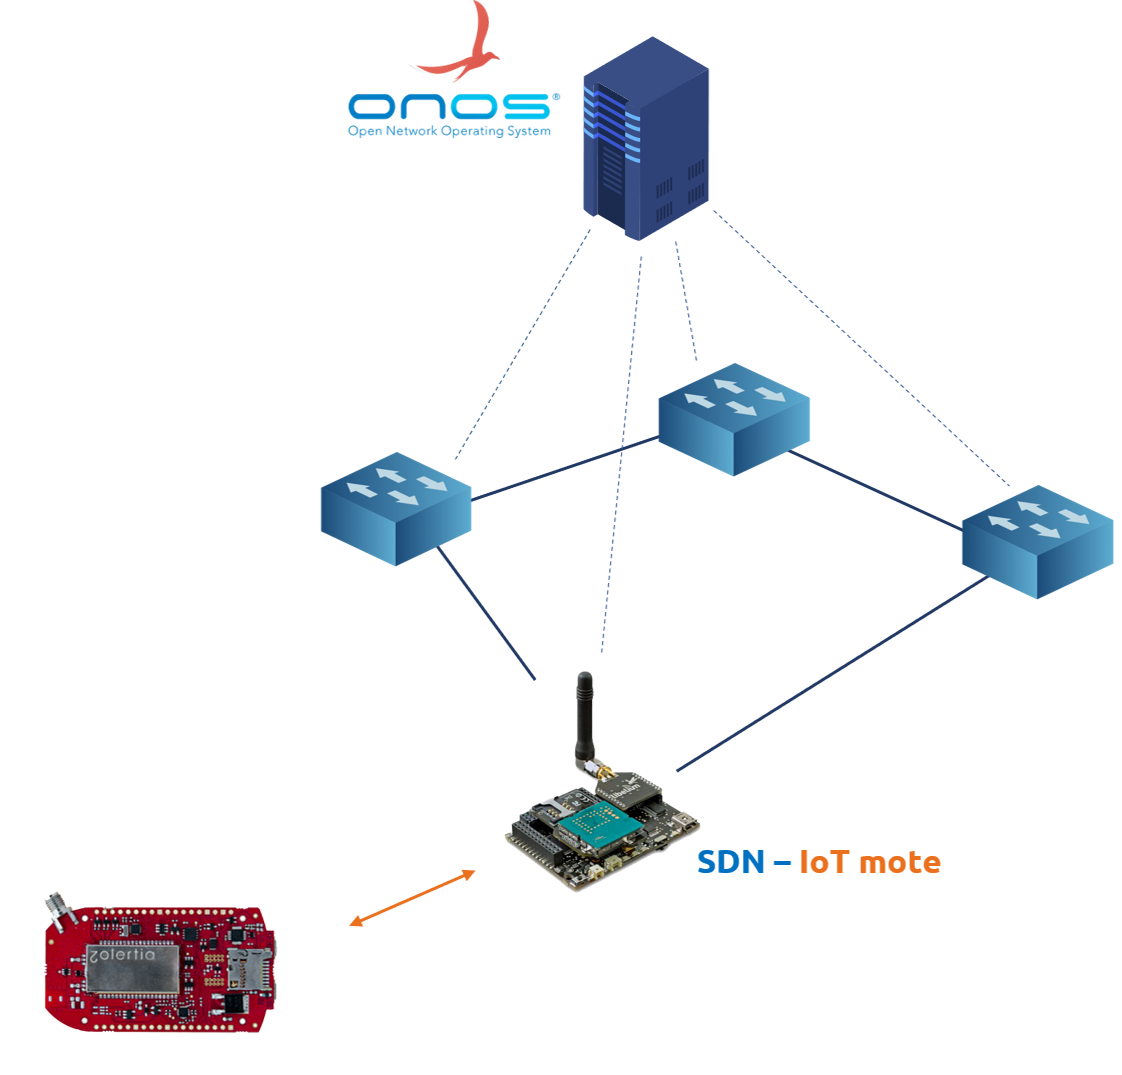
\includegraphics[width=0.7\textwidth]{img/sdn_iot_b.png}
      \caption{Integración total de dispositivos IoT en el core SDN.}
      \label{fig:sdn_iotb}
    \end{figure}
  \end{column}
  
\end{columns}
\end{frame}

%%%%%%%%%%%%%%%%%%%%%%%%%%%%%%%%%%%%%%%%%%%%%%%%%%%%%%%%%%%%%%%%%
\subsection{Tecnologías para la definición del datapath}
\begin{frame}{Introducción}{Tecnologías para la definición del datapath}

\begin{itemize}
    \item El lenguaje \textbf{P4}  permite definir el procesado de los paquetes para un conjunto de arquitecturas que tienen su propia especificación, para conseguir que los programas P4 sean \textbf{independientes del hardware} donde se ejecute. \vspace{0.2cm}

    \item \textbf{XDP} es un framework programable y de \textbf{alto rendimiento} para el procesado de paquetes en el Kernel de Linux. Se lleva a cabo en el punto más bajo de la pila de red de Linux.
\end{itemize}
 \begin{figure}
      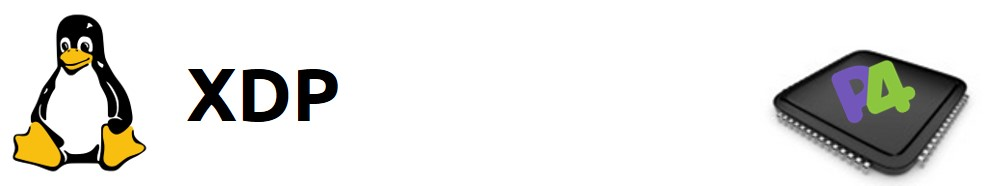
\includegraphics[width=\textwidth]{img/5.jpg}
      \label{fig:datapaths}
    \end{figure}

\end{frame}

%%%%%%%%%%%%%%%%%%%%%%%%%%%%%%%%%%%%%%%%%%%%%%%%%%%%%%%%%%%%%%%%%
\section{Objetivos}
\begin{frame}{Objetivos}

\begin{exampleblock}{Una meta}
El objetivo de este proyecto es realizar un estudio y análisis de las tecnologías P4 y XDP para la \alert{\textbf{integración}} de dispositivos IoT en entornos SDN. \\
\vspace{0.2cm}
Los dispositivos IoT se beneficiarán de la integración con las redes SDN $ \Rightarrow $  la \textbf{flexibilidad} y \textbf{programabilidad} $ \Rightarrow $  correcta gestión y administración de la red.
\end{exampleblock}
\vspace{0.3cm}
Para alcanzar dicho objetivo, se plantearon los siguientes puntos:
\vspace{0.1cm}
\begin{itemize}
    \item Documentación y estudio
    \item Planteamiento de casos de uso típicos y elección de escenarios
    \item Desarrollo de los casos de uso
    \item Evaluación y comprobación de funcionamiento
\end{itemize}

\end{frame}

%%%%%%%%%%%%%%%%%%%%%%%%%%%%%%%%%%%%%%%%%%%%%%%%%%%%%%%%%%%%%%%%%
\section{Análisis y diseño}
\subsection{Funcionalidades básicas}

\begin{frame}{Análisis y diseño}{Funcionalidades básicas}
\begin{table}[]
\centering
\begin{tabular}{|l|l|}
\hline
\rowcolor[HTML]{0046AD} 
\multicolumn{1}{|c|}{\cellcolor[HTML]{0046AD}{\color[HTML]{FFFFFF} \textbf{Funcionalidad básica}}} &
  \multicolumn{1}{c|}{\cellcolor[HTML]{0046AD}{\color[HTML]{FFFFFF} \textbf{Descripción}}} \\ \hline
\textbf{Case01 - Drop} &
  \begin{tabular}[c]{@{}l@{}}En este caso de uso se quiere ver si es posible\\ \alert{descartar} paquetes.\end{tabular} \\ \hline
\textbf{Case02 - Pass} &
  \begin{tabular}[c]{@{}l@{}}Se quiere comprobar si es\\  posible \alert{dejar pasar} los paquetes, sin afectarles\\  el \textit{datapath} programado con la tecnología.\end{tabular} \\ \hline
\textbf{Case03 - Echo server} &
  \begin{tabular}[c]{@{}l@{}}Se desarrollará un servidor el cual\\ \alert{contestará} todos los \texttt{ECHO-Request}\\ que le lleguen.\end{tabular} \\ \hline
\textbf{Case04 - Layer 3 forwarding} &
  \begin{tabular}[c]{@{}l@{}}Con este caso de uso se comprobará qué tan\\ sencillo es \alert{reenviar} paquetes desde una interfaz\\ a otra del dispositivo.\end{tabular} \\ \hline
\textbf{Case05 - Broadcast} &
  \begin{tabular}[c]{@{}l@{}}Con este caso de uso se quería\\  abordar cómo se puede conseguir\\ la \alert{difusión} de un hipotético paquete.\end{tabular} \\ \hline
\end{tabular}
\end{table}

\end{frame}

%%%%%%%%%%%%%%%%%%%%%%%%%%%%%%%%%%%%%%%%%%%%%%%%%%%%%%%%%%%%%%%%%
\subsection{Plataformas de pruebas alámbricas}
\begin{frame}{Análisis y diseño (II)}{Plataformas de pruebas alámbricas}
Para evaluar los desarrollos de XDP y P4 en entornos cableados, se hará uso del estándar
\texttt{ieee8023} (Ethernet).\vspace{0.2cm}
\begin{itemize}
    \item En XDP se hará uso de las \textbf{Network Namespaces}, para definir los nodos independientes de la red, y de \textbf{Veth}, para emular los distintos enlaces.\vspace{0.2cm}\begin{itemize}
        \item La expresión más básica de emulación de redes en el Kernel de Linux.\vspace{0.2cm}
        
        \item La mínima incertidumbre sobre los resultados obtenidos.

    \end{itemize}\vspace{0.2cm}
    \item En P4 se hará uso de \textbf{Mininet}, debido a que el equipo de \textit{p4lang} desarrolló una interfaz del BMv2 con dicha herramienta.
\end{itemize}
\end{frame}

%%%%%%%%%%%%%%%%%%%%%%%%%%%%%%%%%%%%%%%%%%%%%%%%%%%%%%%%%%%%%%%%%
\begin{frame}{Análisis y diseño (II)}{Plataformas de pruebas alámbricas}
\begin{figure}
  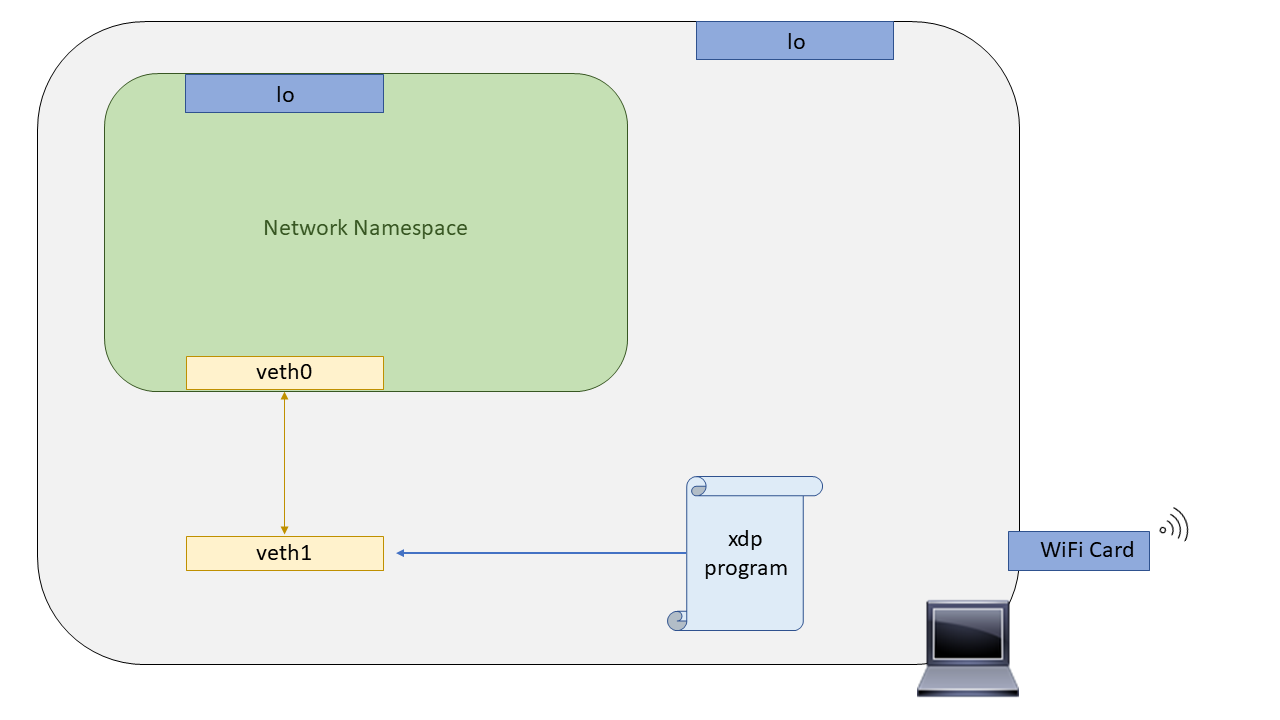
\includegraphics[width=0.9\textwidth]{img/2.png}
  \caption{Escenario entorno cableado XDP.}
  \label{fig:cableados}
\end{figure}
\end{frame}

\begin{frame}{Análisis y diseño (II)}{Plataformas de pruebas alámbricas}
\begin{figure}
  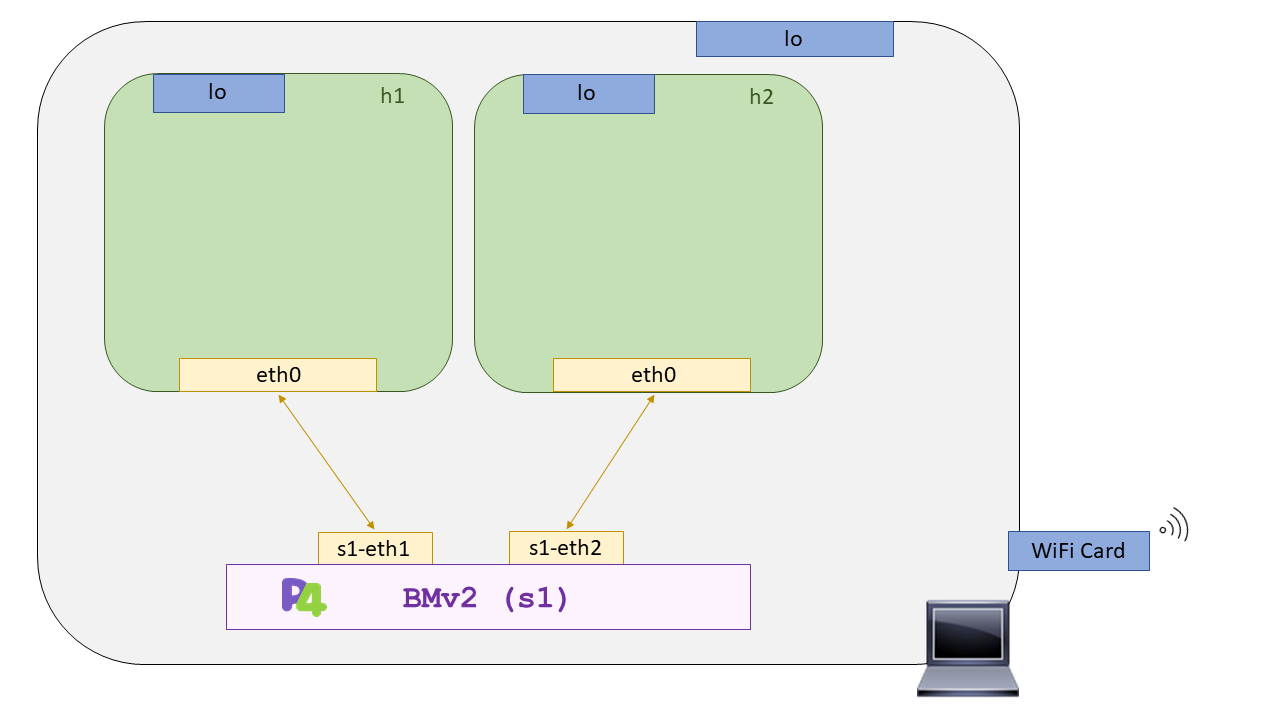
\includegraphics[width=0.9\textwidth]{img/3.png}
  \caption{Escenario entorno cableado P4.}
  \label{fig:cableados2}
\end{figure}
\end{frame}

%%%%%%%%%%%%%%%%%%%%%%%%%%%%%%%%%%%%%%%%%%%%%%%%%%%%%%%%%%%%%%%%%
\subsection{Plataformas de pruebas inalámbricas}
\begin{frame}{Análisis y diseño (III)}{Plataformas de pruebas inalámbricas}
\justify{
En entornos inalámbricos se hará uso del estándar \textbf{\texttt{ieee80211}} (WiFi). Se ha elegido dicho estándar dado que existen más herramientas y desarrollos que para el estándar \texttt{ieee802154}.}\vspace{0.2cm}
\begin{itemize}
    \item  La plataforma que se utilizará para la evaluación de los distintos casos de uso, tanto en XDP como en P4, será la misma, \textbf{Mininet-WiFi}. \vspace{0.2cm}\begin{itemize}
        \item[] \cmark \hspace{0.1cm} Posibilidad de hacer uso de las funcionalidades de Mininet-IoT\vspace{0.1cm}
        \item[] \alert{\xmark} \hspace{0.1cm} No es viable utilizar el simulador Cooja 
    \end{itemize}
    
\end{itemize}\vspace{0.2cm}

\begin{columns}

  \begin{column}{0.9\textwidth}
    Pero, se ha visto que la plataforma \alert{no contempla} ningún tipo de nodo que de soporte \alert{al BMv2} por lo que será necesario desarrollar previamente una integración del BMv2 en Mininet-WiFi.
        
  \end{column}
  
  \begin{column}{0.1\textwidth}  %%<--- here
      \begin{figure}
      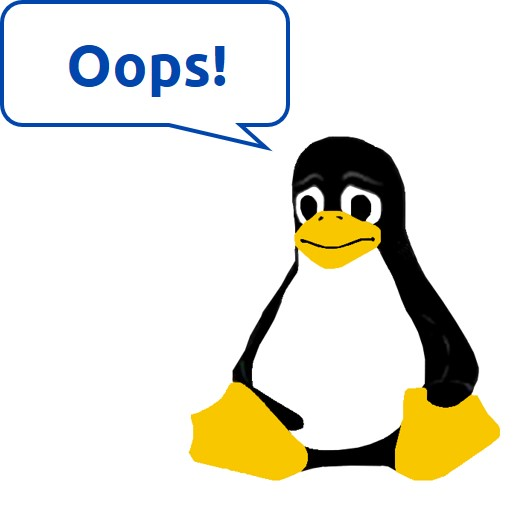
\includegraphics[width=1.3\textwidth]{img/4.jpg}
      \end{figure}
  \end{column}
  
\end{columns}

\end{frame}


%%%%%%%%%%%%%%%%%%%%%%%%%%%%%%%%%%%%%%%%%%%%%%%%%%%%%%%%%%%%%%%%%
\section{Desarrollo}
\subsection{Medios Cableados}
\begin{frame}{Desarrollo}{Medios Cableados}
\begin{itemize}
    \item \textbf{case01 - Drop}: Con XDP se uso de código de retorno \texttt{XDP\_DROP}. Con P4, se uso la primitiva \texttt{mark\_to\_drop()}.\vspace{0.3cm}
    
    \item \textbf{case02 - Pass}: con XDP se pudo implementar haciendo uso del código de retorno \texttt{XDP\_PASS}.\vspace{0.2cm}
    \begin{itemize}
        \item[] \alert{\xmark} \hspace{0.1cm} Con P4, no se pudo implementar. Se debe definir de forma exclusiva todo el \textit{datapath}. 
    \end{itemize}\vspace{0.3cm}
    \item \textbf{case03 - Echo server}: Se filtraron los paquetes, y en base al tipo de paquete, se aplicaron unas acciones u otras.\vspace{0.2cm}
    \begin{itemize}
        \item[] \cmark  \hspace{0.1cm} \texttt{XDP\_TX}\vspace{0.1cm}
        \item[] \cmark  \hspace{0.1cm} \texttt{standard\_metadata.egress\_spec} 
    \end{itemize}
\end{itemize}
\end{frame}

%%%%%%%%%%%%%%%%%%%%%%%%%%%%%%%%%%%%%%%%%%%%%%%%%%%%%%%%%%%%%%%%%
\begin{frame}{Desarrollo}{Medios Cableados}
\begin{itemize}
    \item \textbf{case04 -  Layer 3 forwarding}:  Con XDP se exploraron distintas formas de hacer forwarding haciendo uso de los \textbf{BPF Helpers}, desde la más sencilla y más estática, a una donde se trabajaba de forma colaborativa con  el Kernel.
\end{itemize}

\begin{figure}
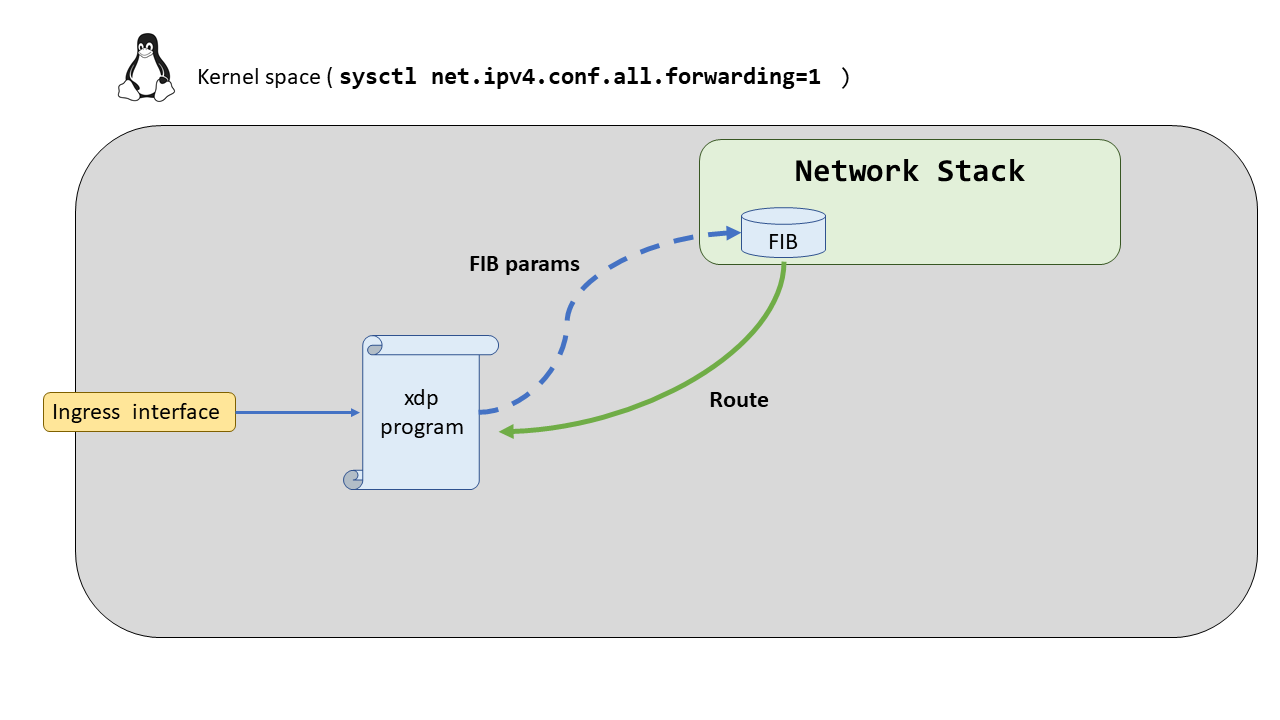
\includegraphics[width=0.7\textwidth]{img/6.png}
\caption{Forwarding Auto}
\end{figure}
        


\end{frame}

%%%%%%%%%%%%%%%%%%%%%%%%%%%%%%%%%%%%%%%%%%%%%%%%%%%%%%%%%%%%%%%%%
\begin{frame}{Desarrollo}{Medios Cableados}

\begin{block}{Forwarding en P4}
 \vspace{-0.2cm}
 \lstinputlisting[style=P4-color]{code/p4.c}
\end{block}
\end{frame}

%%%%%%%%%%%%%%%%%%%%%%%%%%%%%%%%%%%%%%%%%%%%%%%%%%%%%%%%%%%%%%%%%
\begin{frame}{Desarrollo}{Medios Cableados}
\begin{itemize}
    \item \textbf{case05 - Broadcast}:  Con P4 se llevó a cabo el broadcast haciendo uso de los grupos multicast (JSON donde se definían las replicas). Con XDP no se pudo utilizar el \textit{helper} BPF para la clonación del paquete ya que requería hacer uso de la estructura \texttt{sk\_buff}.
\end{itemize}

\begin{figure}
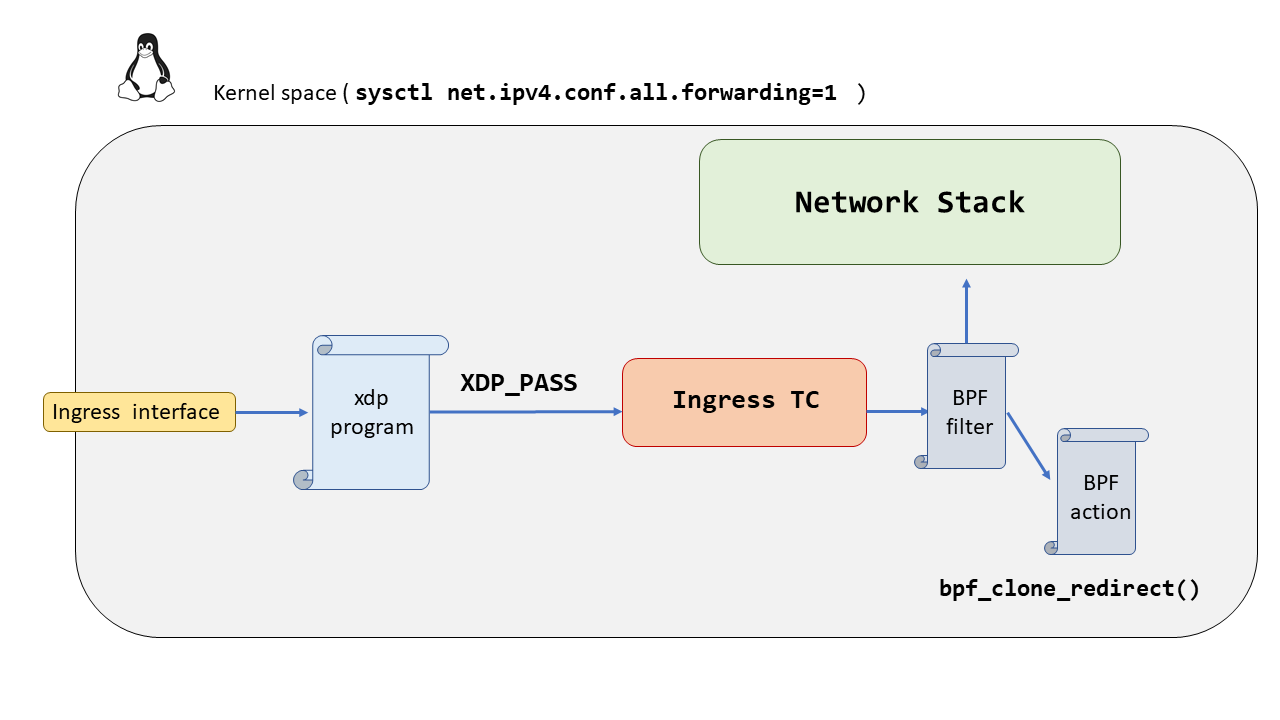
\includegraphics[width=0.85\textwidth]{img/7.png}
\end{figure}

\end{frame}

%%%%%%%%%%%%%%%%%%%%%%%%%%%%%%%%%%%%%%%%%%%%%%%%%%%%%%%%%%%%%%%%%
\subsection{Medios Inalámbricos}
\begin{frame}{Desarrollo}{Medios Inalámbricos}
El primer paso en el desarrollo de los casos de uso en medios inalámbricos pasa por la integración del BMv2 en Mininet-Wifi.\vspace{0.2cm}

\begin{figure}
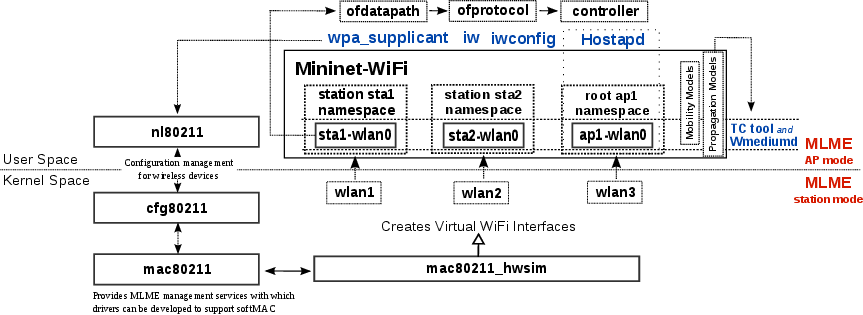
\includegraphics[width=0.85\textwidth]{img/mininet_wifi_components.png}
\end{figure}
\end{frame}

%%%%%%%%%%%%%%%%%%%%%%%%%%%%%%%%%%%%%%%%%%%%%%%%%%%%%%%%%%%%%%%%%
\begin{frame}{Desarrollo}{Medios Inalámbricos}

\begin{columns}

  \begin{column}{0.5\textwidth}
    \begin{figure}
      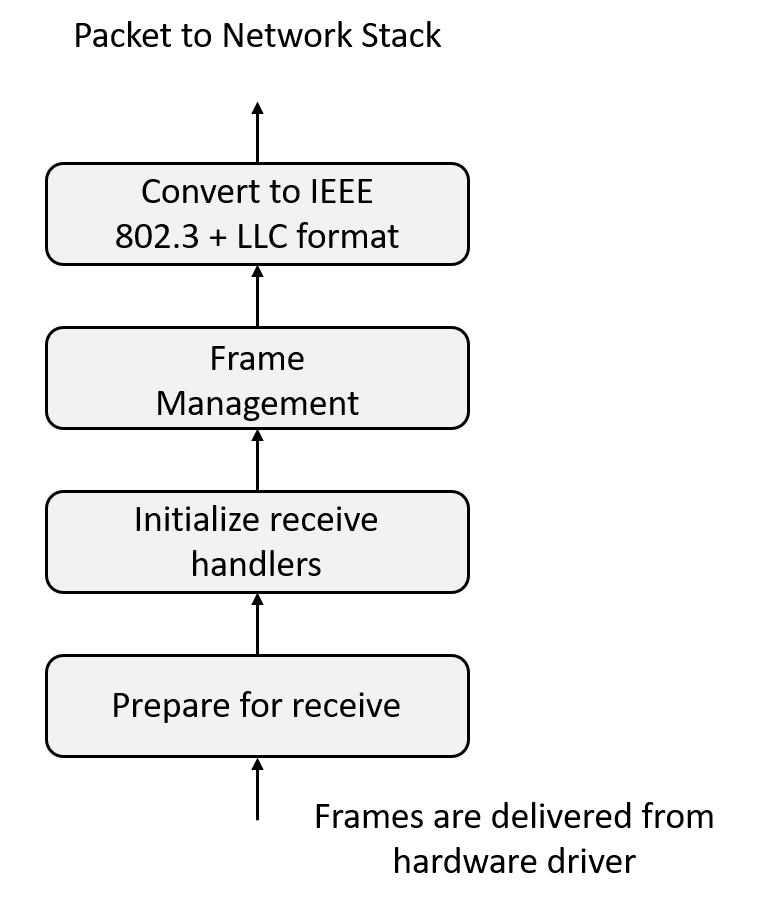
\includegraphics[width=0.8\textwidth]{img/linux_wireless_subsystem_rx.png}
      \caption{ Flujo para la recepción con el módulo mac80211\_hwsim}
      \label{fig:a}
    \end{figure}
        
  \end{column}
  \vrule\hspace{0.4cm}
  \begin{column}{0.5\textwidth}  %%<--- here
     \begin{figure}
      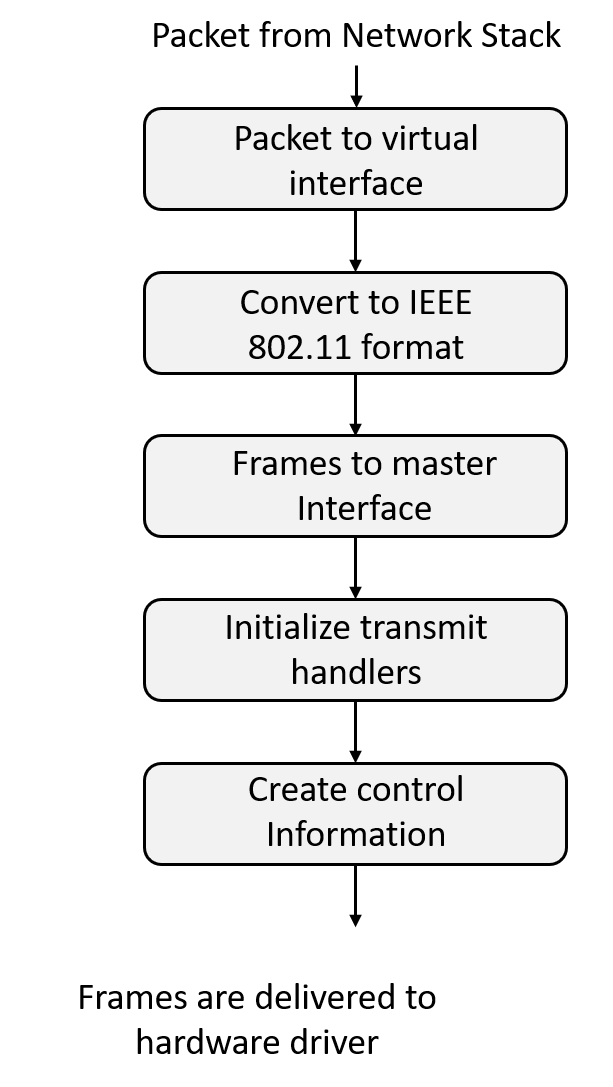
\includegraphics[width=0.52\textwidth]{img/linux_wireless_subsystem_tx.png}
      \caption{Flujo para la transmisión con el módulo mac80211\_hwsim}
      \label{fig:b}
    \end{figure}
  \end{column}
  
\end{columns}

\end{frame}

%%%%%%%%%%%%%%%%%%%%%%%%%%%%%%%%%%%%%%%%%%%%%%%%%%%%%%%%%%%%%%%%%
\begin{frame}{Desarrollo}{Medios Inalámbricos}

\begin{figure}
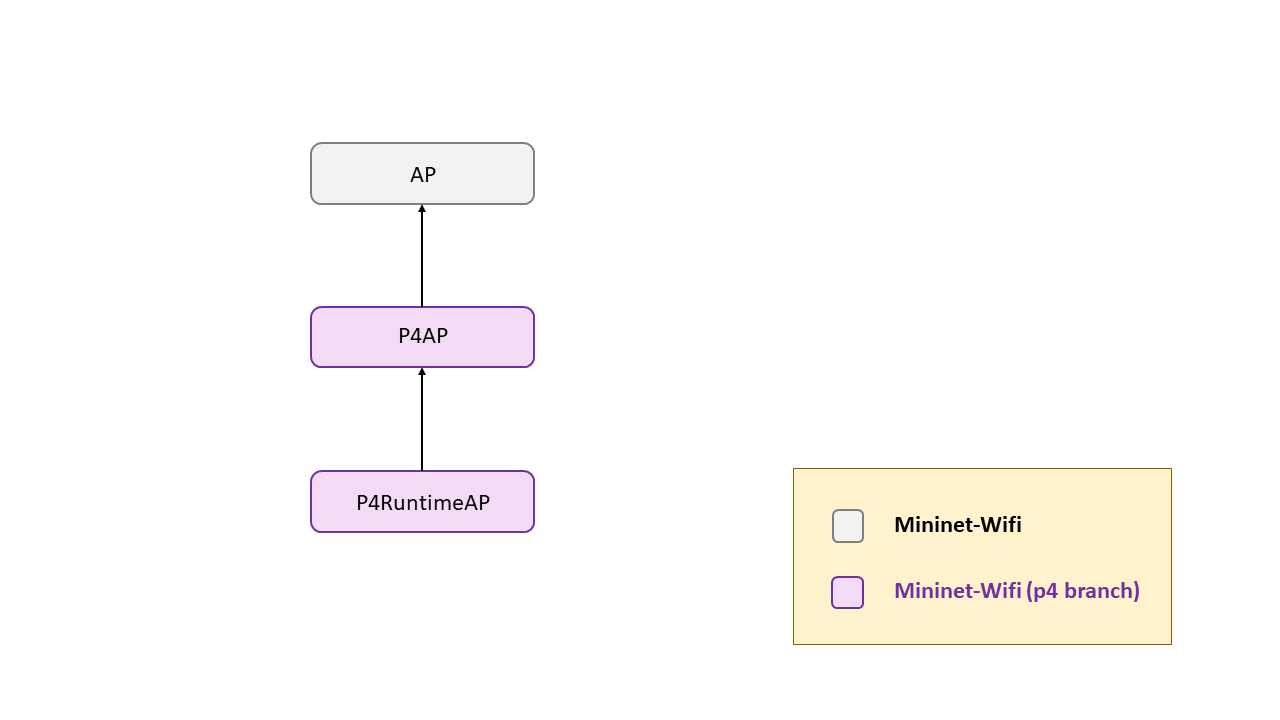
\includegraphics[width=0.9\textwidth]{img/p4_Mininet_Wifi_UML.png}
\caption{UML de la integración BMv2 con Mininet-WiFi}
\end{figure}

\end{frame}

%%%%%%%%%%%%%%%%%%%%%%%%%%%%%%%%%%%%%%%%%%%%%%%%%%%%%%%%%%%%%%%%%
\begin{frame}{Desarrollo}{Medios Inalámbricos}

\begin{block}{Limitación inducida por el propio módulo}
 Al trabajar de nuevo con Ethernet, la mayoría de casos de uso son operativos en medios inalámbricos. En caso de manejar las cabeceras WiFi, únicamente habría que cambiar las etapas de \textit{parsing} y gestión de cabeceras.
\end{block}
\vspace{0.2cm}
Hay casos de uso que se benefician de este nuevo medio, como por ejemplo: \textbf{case05 - Broadcast} en XDP.\vspace{0.2cm}
\begin{itemize}
    \item Esto se debe a que el medio es compartido, solo hay una tarjeta wireless emulada. Por tanto, para para difundir únicamente debe\textbf{ modificar las cabeceras a difusión} y \textbf{retransmitir} por la misma interfaz por la cual llego el paquete, \textbf{\texttt{XDP\_TX}}.\vspace{0.2cm}
\end{itemize}
\end{frame}

%%%%%%%%%%%%%%%%%%%%%%%%%%%%%%%%%%%%%%%%%%%%%%%%%%%%%%%%%%%%%%%%%
\section{Conclusiones}

\begin{frame}{Conclusiones}
\begin{itemize}
    \item  XDP, está mejor enfocado para escenarios de integración totales. Se beneficiará del rendimiento y la optimización de recursos que ofrece XDP.\vspace{0.2cm}
    
    \item Tecnología P4, está más enfocada a escenarios de integración parcial. Se beneficiarán de las facilidades para realizar multicast, y de su interfaz de control.
\end{itemize}
\vspace{0.2cm}

\begin{table}[ht]
\centering
\begin{tabular}{|l|c|c|c|c|}
\hline
\rowcolor[HTML]{0046AD} 
{\color[HTML]{FFFFFF} \textbf{Caso de uso}} &
  {\color[HTML]{FFFFFF} \textbf{XDP}} &
  {\color[HTML]{FFFFFF} \textbf{P4}} &
  {\color[HTML]{FFFFFF} \textbf{P4-Wireless}} &
  {\color[HTML]{FFFFFF} \textbf{XDP-Wireless}} \\ \hline
case01 - Drop               & \cmark         & \cmark         & \cmark         & \cmark \\ \hline
case02 - Pass               & \cmark         & \alert{\xmark} & \alert{\xmark} & \cmark \\ \hline
case03 - Echo server        & \cmark         & \cmark         & \cmark         & \cmark \\ \hline
case04 - Layer 3 forwarding & \cmark         & \cmark         & \cmark         & \cmark \\ \hline
case05 - Broadcast          & \alert{\xmark} & \cmark         & \cmark         & \cmark \\ \hline
\end{tabular}
\caption{Resumen sobre los casos de uso desarrollados}
\label{tab:useCases}
\end{table}
\end{frame}

%%%%%%%%%%%%%%%%%%%%%%%%%%%%%%%%%%%%%%%%%%%%%%%%%%%%%%%%%%%%%%%%%
\section{Trabajo Futuro}
\subsection{Integración de interfaces en modo monitor con los casos de uso}
\begin{frame}{Trabajo Futuro}{Integración de interfaces en modo monitor con los casos de uso}

\begin{columns}

  \begin{column}{0.6\textwidth}
  \justify{
    No se ha podido gestionar de forma directa los paquetes con las cabeceras WiFi. Las interfaces creadas por este módulo operan con Ethernet, el único modo que opera con las cabeceras WiFi es en el modo \textbf{monitor}.}
    \vspace{0.4cm}
    \begin{itemize}
        \item Pero el modo monitor está pensado únicamente para escuchar paquetes, no para transmitir.\vspace{0.2cm}
        \item Este modo puede ser llevado al límite haciendo un \alert{\textit{packet injection}}.
    \end{itemize}
    
  \end{column}
  
  \begin{column}{0.4\textwidth}  %%<--- here
   \begin{figure}
    \centering
    \begin{tikzpicture}[node distance=1.5cm, auto]
    	% Cuadros
    	\node (deps) [rectnaranja,text width=4cm] {\texttt{Scapy (WiFi Headers)} \par};
    	\node (deps2) [rectverde,below of=deps,text width=3cm] { \texttt{Socket raw} \par};
    	\node (harddep) [rectvioleta,below of=deps2,text width=3cm]{ \texttt{Transmitir el paquete} \par};
    	% Flechas
        \draw[arrow] (deps) -- (deps2);
        \draw[arrow] (deps2) -- (harddep);
    
    \end{tikzpicture}
    \caption{Flujo de inyección de paquetes.}
    \label{fig:DependenciasIproute}
    \end{figure}
  \end{column}
  
\end{columns}

\end{frame}

%%%%%%%%%%%%%%%%%%%%%%%%%%%%%%%%%%%%%%%%%%%%%%%%%%%%%%%%%%%%%%%%%
\subsection{Emulación de redes de baja capacidad - mac802154\_hwsim}
\begin{frame}{Trabajo Futuro}{Emulación de redes de baja capacidad - mac802154\_hwsim}
\begin{block}{Un paso  más en la integración...}
 Explorar las fortalezas y debilidades, tanto de XDP como de P4, en la definición del \textit{datapath} de dispositivos de \textbf{baja capacidad}. \\
 \vspace{0.2cm}
 Estos necesitarán que la tecnología que defina su \textit{datapath} sea lo más \alert{\textbf{eficiente}} posible, haciendo un uso \alert{\textbf{optimizado}} de los recursos de la mota IoT.
\end{block}

\begin{figure}
  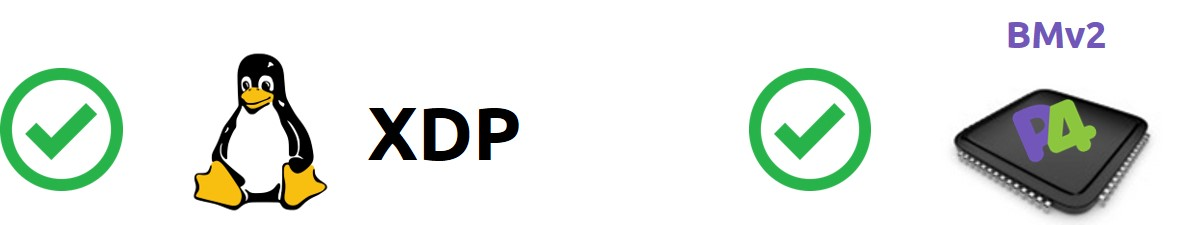
\includegraphics[width=\textwidth]{img/1_test.jpg}
  \label{fig:future}
\end{figure}
\end{frame}

%%%%%%%%%%%%%%%%%%%%%%%%%%%%%%%%%%%%%%%%%%%%%%%%%%%%%%%%%%%%%%%%%
{\disableNavigation{white}
    \begin{frame}{}
       \begin{figure}
              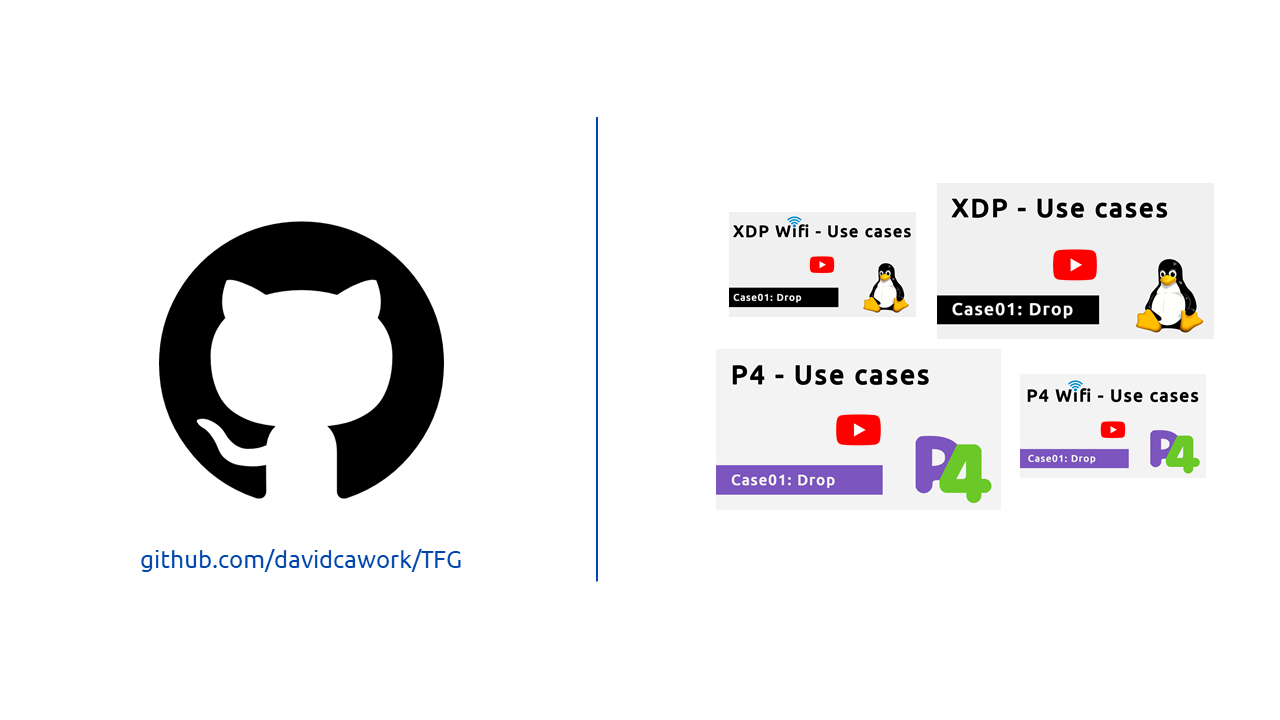
\includegraphics[width=\textwidth]{img/init.png}
        \end{figure}
    \end{frame}
}


%%%%%%%%%%%%%%%%%%%%%%%%%%%%%%%%%%%%%%%%%%%%%%%%%%%%%%%%%%%%%%%%%
\section{¿Preguntas?}
{
\sectionheaderWhite 

\begin{frame}{¡Muchas gracias por su atención!}{¿Preguntas?}
\end{frame}

}


\end{document}
